\documentclass[12pt,a4paper]{article}
\usepackage[utf8]{inputenc}
\usepackage[english]{babel}
%\usepackage{minted}
\usepackage{listings}
\usepackage{xcolor}
\usepackage{graphicx}

%For syntax highlighting
\definecolor{codegreen}{rgb}{0,0.6,0}
\definecolor{codegray}{rgb}{0.5,0.5,0.5}
\definecolor{codepurple}{rgb}{0.58,0,0.82}
\definecolor{backcolour}{rgb}{1,1,1}

%%Sets different parameters
\lstdefinestyle{mystyle}{
	backgroundcolor=\color{backcolour},   
    commentstyle=\color{codegreen},
    keywordstyle=\color{magenta},
    numberstyle=\tiny\color{codegray},
    stringstyle=\color{codepurple},
    basicstyle=\ttfamily\footnotesize,
    breakatwhitespace=false,         
    breaklines=true,                 
    captionpos=b,                    
    keepspaces=true,                 
    numbers=left,                    
    numbersep=5pt,                  
    showspaces=false,                
    showstringspaces=false,
    showtabs=false,                  
    tabsize=4
}
\lstset{style=mystyle}

\title{\bf 16 Bit Arithmetic Operations}
\author{\vspace{-10ex}}
\date{\vspace{-10ex}}
\begin{document}
\maketitle

\begin{minipage}{0.45\textwidth}
        \begin{tabular}{l l}
            \textbf{Expt No:}&2\\
            \textbf{Date :}&28/08/2020
        \end{tabular}
\end{minipage}%
\begin{minipage}{0.45\textwidth}
        \begin{tabular}{l l}
             \textbf{Name:}& Shivanirudh S G  \\
             \textbf{Reg No:} & 185001146 
        \end{tabular}
\end{minipage}
\vspace{1cm}
\hrule

\begin{flushleft}
\subsection*{\textbf{Aim:}} 
To perform arithmetic operations on two 16 bit numbers.

\vspace{1cm}
\hrule
\subsection*{\textbf{\underline{16 Bit Addition}}}

\subsubsection*{\textbf{Algorithm:}}
\begin{itemize}
    \item Move the data segment to the AX register and then move it to the DS register.
    \item Move the first operand to AX register. 
    \item Move the second operand to the BX register. 
    \item Initially set the CX register to 0000h. 
    \item Then add using ADD AX,BX.
    \item Using JNC instruction check for carry and if there is no carry, no need to increment CX.
    \item Else, increment CX by 1. 
    \item The result and carry stored in AX and CX should be moved to RESULT
and CARRY respectively.
\end{itemize}

\newpage
\subsubsection*{\textbf{Program:}}

\begin{table}[htb]
\centering
\resizebox{\columnwidth}{!}{
\begin{tabular}{|l|l|} 
\hline
\textbf{Program}                                                 & \textbf{Comments}                             \\ 
\hline
\hline
assume cs:code,ds:data                                           & Declare code and data segments                \\
\hline
data segment                                                     & Start of data segment                         \\
\hline 
opr1 db 1111h                                                    & Define byte opr1 with hex value 1111          \\
\hline
opr2 db 9999h                                                    & Define byte opr2 with hex value 9999          \\
\hline
result db 0000H                                                  & Define byte result with hex value 0000        \\
\hline
carry db 0000H                                                   & Define byte carry with hex value 0000         \\
\hline      
data ends                                                        & End of data segment                           \\
\hline
code segment                                                     & Start of code segment                         \\
\hline
org 0100h                                                        & Set preferred offset                          \\
\hline
start:~ mov ax,data                                              & Move data segment contents to AX register     \\ 
\hline
mov ds,ax                                                        & Move data in AX register to DS register       \\ 
\hline
mov ax,opr1                                                      & Move contents of opr1 to AX register          \\ 
\hline
mov bx,opr2                                                      & Move contents of opr2 to BX register          \\ 
\hline
mov cx,00h                                                       & Move hex value 00 to CX register              \\ 
\hline
add ax,bx                                                        & AH = AX + BX                                  \\ 
\hline
jnc here                                                         & Jump to the label here, if there is no carry  \\ 
\hline
inc cx                                                           & Increment value of CX if there is a carry     \\ 
\hline
here:~ mov result,ax                                             & Move contents of AX register to result        \\ 
\hline
mov carry,cx                                                     & Move contents of CX register to carry         \\ 
\hline
int 21h                                                          & Request interrupt routine                     \\ 
\hline
code ends                                                        & End of code segment                           \\
\hline
end start                                                        &                                               \\
\hline
\end{tabular}
}
\end{table}

\newpage
\subsection*{\textbf{Unassembled code:}}
\begin{figure}[h]
    \centering
    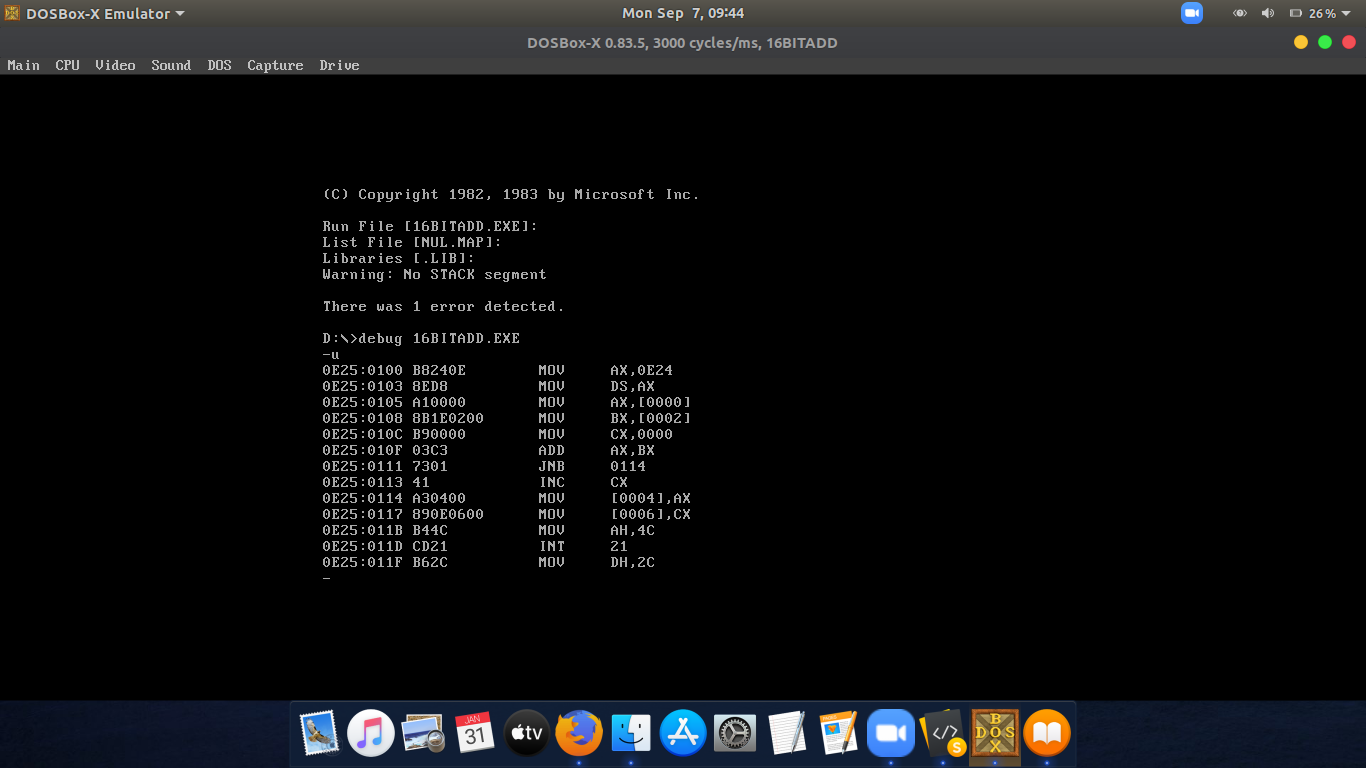
\includegraphics[trim = 100mm 60mm 150mm 127mm, clip, width = \textwidth]{Pics/AdditionUS.png}
\end{figure}
\subsubsection*{\textbf{Input and Output:}}
\begin{figure}[h]
    \centering
    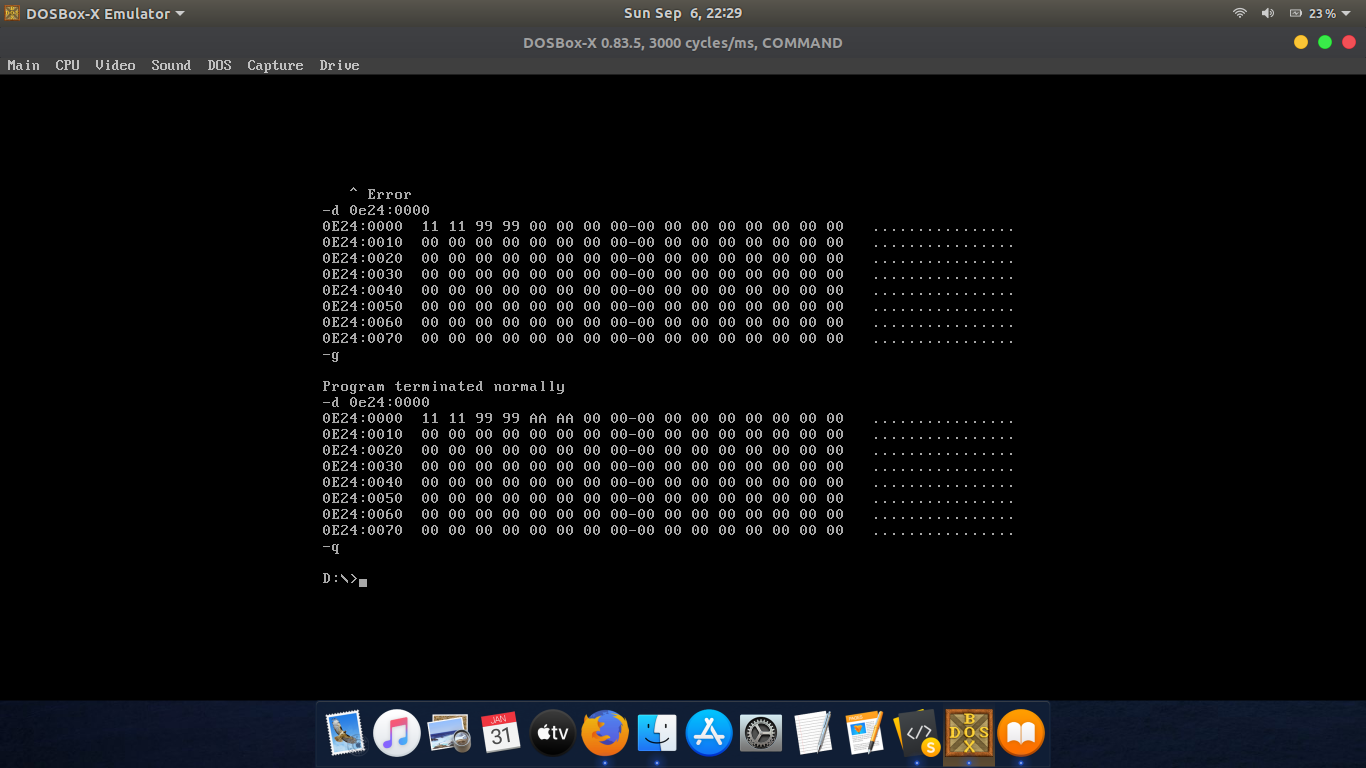
\includegraphics[trim = 100mm 75mm 100mm 70mm, clip, width = \textwidth]{Pics/AdditionIO.png}
    \caption{ \textbf{Input:} \emph{opr1:} 1111h, \emph{opr2:} 9999h; 
              \textbf{Output:} \emph{Result:} AAAAh, \emph{Carry:} 0000h}
\end{figure}
%--------------------------------------------------------------------------------------------------------------------------------------------
\newpage
\subsection*{\textbf{\underline{16 Bit Subtraction}}}

\subsubsection*{\textbf{Algorithm:}}
\begin{itemize}
    \item Move the data segment to the AX register and then move it to the DS register.
    \item Move the first operand to AX register. 
    \item Move the second operand to the BX register. 
    \item Initially set the CX register to 0000h. 
    \item Then subtract using SUB AX,BX.
    \item Check for carry using JNC instruction. If no carry then it means AX $>$ BX and hence no need to increment CX and no need to complement AX.
\item Else, AX$<$BX. Hence we have to take 2’s complement of AX using NEG AX and also increment CX by 1 using INC CX.
\item The result and carry stored in AX and CX should be moved to RESULT and CARRY respectively.
\end{itemize}

\newpage
\subsubsection*{\textbf{Program:}}

\begin{table}[htb]
\centering
\resizebox{\columnwidth}{!}{
\begin{tabular}{|l|l|} 
\hline
\textbf{Program}                                                 & \textbf{Comments}                             \\ 
\hline
\hline
assume cs:code,ds:data                                           & Declare code and data segments                \\
\hline
data segment                                                     & Start of data segment                         \\
\hline 
opr1 db 1111h                                                    & Define byte opr1 with hex value 1111          \\
\hline
opr2 db 9999h                                                    & Define byte opr2 with hex value 9999          \\
\hline
result db 0000H                                                  & Define byte result with hex value 0000        \\
\hline
carry db 0000H                                                   & Define byte carry with hex value 0000         \\
\hline      
data ends                                                        & End of data segment                           \\
\hline
code segment                                                     & Start of code segment                         \\
\hline
org 0100h                                                        & Set preferred offset                          \\
\hline
start:~ mov ax,data                                              & Move data segment contents to AX register     \\ 
\hline
mov ds,ax                                                        & Move data in AX register to DS register       \\ 
\hline
mov ax,opr1                                                      & Move contents of opr1 to AX register          \\ 
\hline
mov bx,opr2                                                      & Move contents of opr2 to BX register          \\ 
\hline
mov cx,00h                                                       & Move hex value 00 to CX register              \\ 
\hline
sub ax,bx                                                        & AH = AX + BX                                  \\ 
\hline
jnc here                                                         & Jump to the label here, if there is no carry  \\ 
\hline
inc cx                                                           & Increment value of CX if there is a carry     \\ 
\hline
neg ax                                                           & Negate value of AX if there is a carry        \\
\hline
here:~ mov result,ax                                             & Move contents of AX register to result        \\ 
\hline
mov carry,cx                                                     & Move contents of CX register to carry         \\ 
\hline
int 21h                                                          & Request interrupt routine                     \\ 
\hline
code ends                                                        & End of code segment                           \\
\hline
end start                                                        &                                               \\
\hline
\end{tabular}
}
\end{table}

\newpage
\subsection*{\textbf{Unassembled code:}}
\begin{figure}[h]
    \centering
    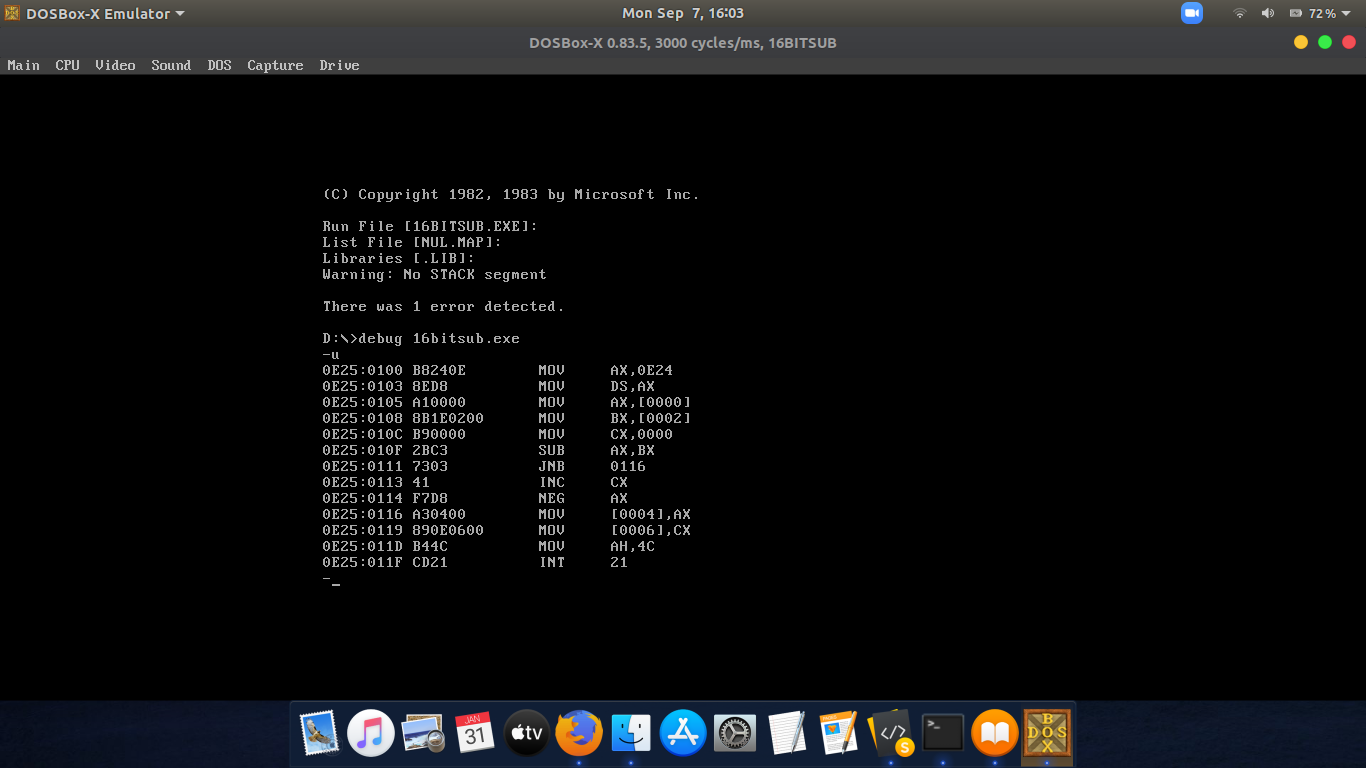
\includegraphics[trim = 100mm 60mm 150mm 127mm, clip, width = \textwidth]{Pics/SubtractionUS.png}
\end{figure}
\subsubsection*{\textbf{Input and Output:}}
\begin{figure}[h]
    \centering
    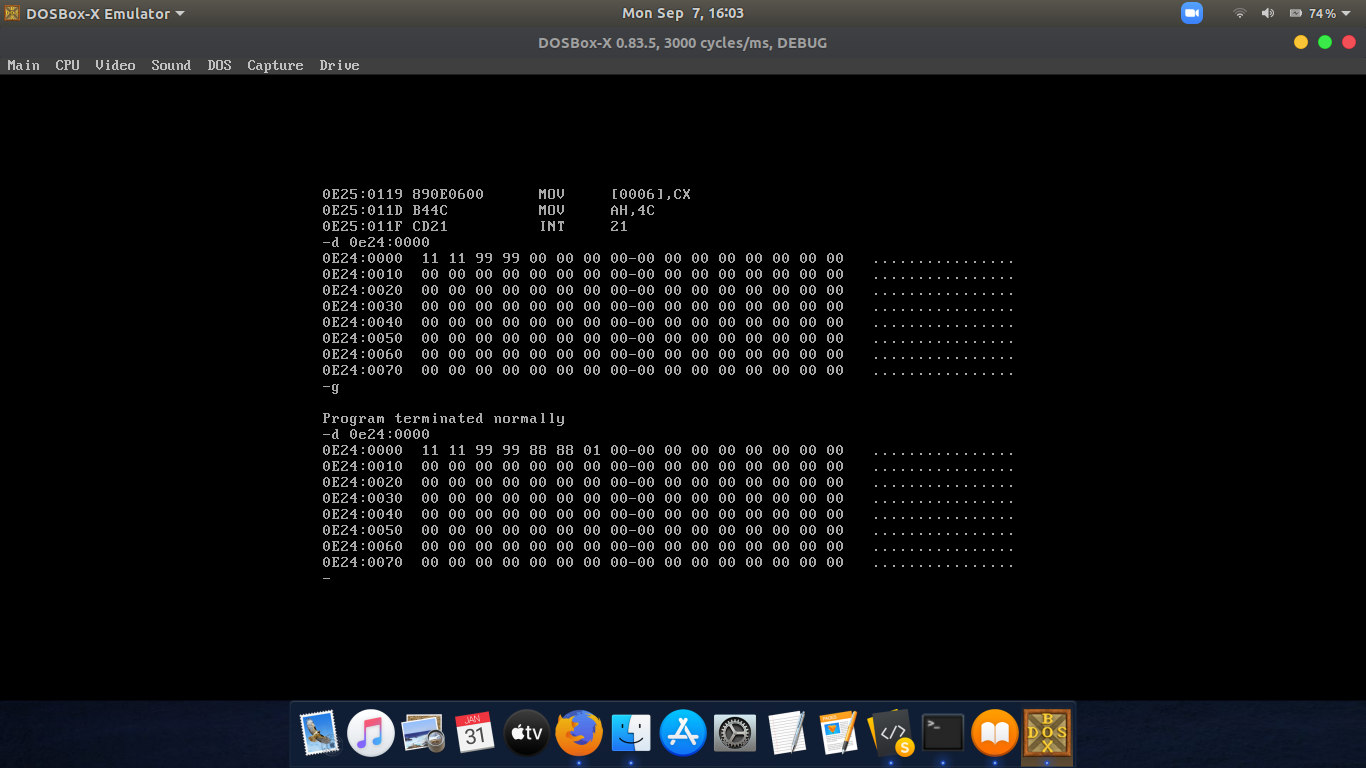
\includegraphics[trim = 100mm 60mm 100mm 80mm, clip, width = \textwidth]{Pics/SubtractionIO.png}
    \caption{ \textbf{Input:} \emph{opr1:} 1111h, \emph{opr2:} 9999h; 
              \textbf{Output:} \emph{Result:} 8888h, \emph{Sign:} 0001h}
\end{figure}

%--------------------------------------------------------------------------------------------------------------------------------------------
\newpage
\subsection*{\textbf{\underline{16 Bit Multiplication}}}

\subsubsection*{\textbf{Algorithm:}}
\begin{itemize}
    \item Move the data segment to the AX register and then move it to the DS register.
    \item Move the first operand to AX register.
    \item  Move the second operand to the BX register.
    \item  Then multiply using MUL BX.(Since AL is default operand register for MUL instruction we only need to specify the other operand register.)
    \item  The result stored in (DX)(AX) register(32 bit- because multiplication of two 16 bit numbers yields a 32 bit number) should now be moved to RESULT.
\end{itemize}

\newpage
\subsubsection*{\textbf{Program:}}
\begin{table}[htb]
\centering\small
\resizebox{\columnwidth}{!}{
\begin{tabular}{|l|l|} 
\hline
\textbf{Program}                                                 & \textbf{Comments}                             \\ 
\hline
\hline
assume cs:code,ds:data                                           & Declare code and data segments                \\
\hline
data segment                                                     & Start of data segment                         \\
\hline 
opr1 db 2222h                                                    & Define byte opr1 with hex value 2222          \\
\hline
opr2 db 3333h                                                    & Define byte opr2 with hex value 3333          \\
\hline
resulth db 0000H                                                 & Define byte resulth with hex value 0000       \\
\hline
resultl db 0000H                                                 & Define byte resultl with hex value 0000       \\
\hline      
data ends                                                        & End of data segment                           \\
\hline
code segment                                                     & Start of code segment                         \\
\hline
org 0100h                                                        & Set preferred offset                          \\
\hline
start:~ mov ax,data                                              & Move data segment contents to AX register     \\ 
\hline
mov ds,ax                                                        & Move data in AX register to DS register       \\ 
\hline
mov ax,opr1                                                      & Move contents of opr1 to AX register          \\ 
\hline
mov dx, 0000H                                                    & Move hex value 0000 to DX register            \\
\hline
mov bx,opr2                                                      & Move contents of opr2 to BX register          \\ 
\hline
mul bx                                                           & (DX)(AX) = AX * BX                            \\ 
\hline
here:~ mov resulth,dx                                            & Move contents of DX register to resulth       \\ 
\hline
mov resultl,ax                                                   & Move contents of AX register to resultl       \\ 
\hline
int 21h                                                          & Request interrupt routine                     \\ 
\hline
code ends                                                        & End of code segment                           \\
\hline
end start                                                        &                                               \\
\hline
\end{tabular}
}
\end{table}

\newpage
\subsection*{\textbf{Unassembled code:}}
\begin{figure}[h]
    \centering
    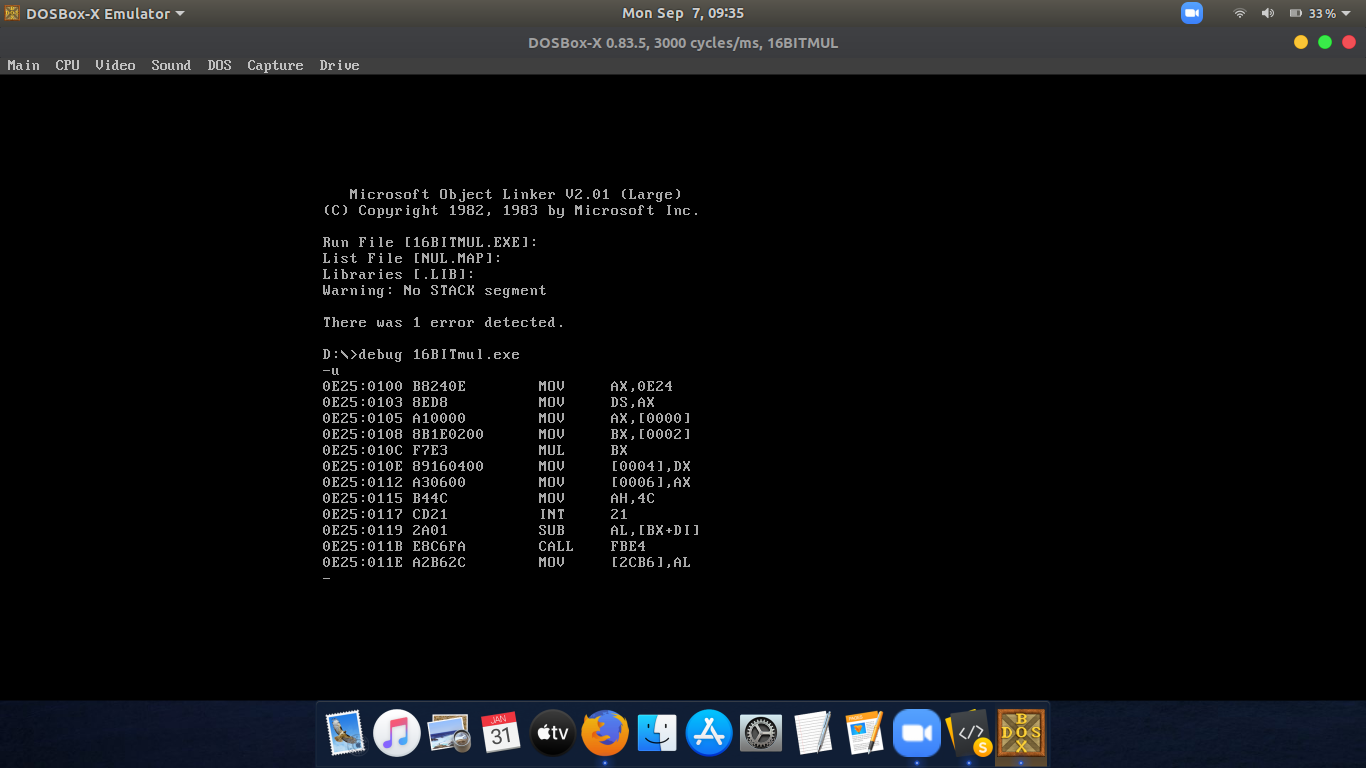
\includegraphics[trim = 100mm 60mm 150mm 127mm, clip, width = \textwidth]{Pics/MultiplicationUS.png}
\end{figure}
\subsubsection*{\textbf{Input and Output:}}
\begin{figure}[h]
    \centering
    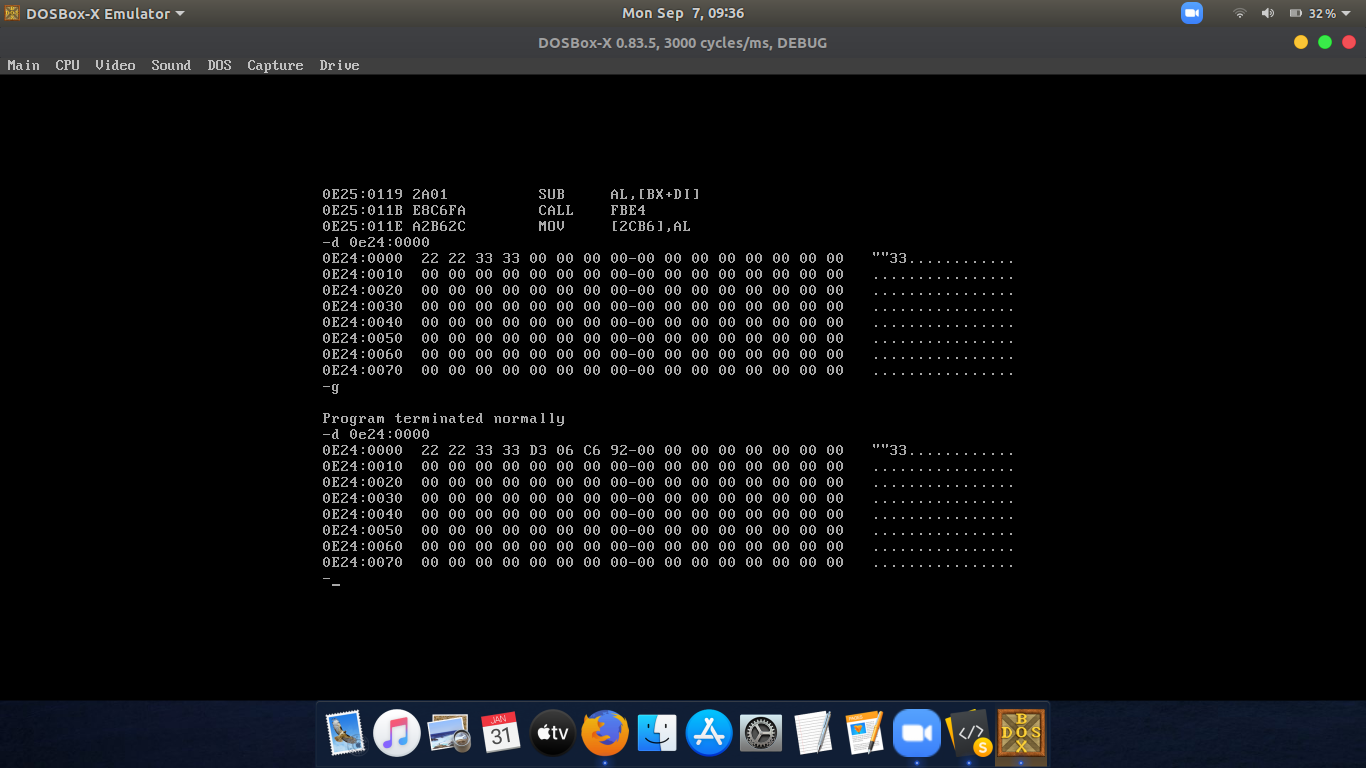
\includegraphics[trim = 100mm 60mm 100mm 80mm, clip, width = \textwidth]{Pics/MultiplicationIO.png}
    \caption{ \textbf{Input:} \emph{opr1:} 2222h, \emph{opr2:} 3333h; 
              \textbf{Output:} \emph{Result:} 92C6 06D3h}
\end{figure}
%--------------------------------------------------------------------------------------------------------------------------------------------
\newpage
\subsection*{\textbf{\underline{16 Bit Division}}}

\subsubsection*{\textbf{Algorithm:}}
\begin{itemize}
    \item Move the data segment to the AX register and then move it to the DS register.
    \item Move the first operand to AX register.
    \item  Move the second operand to the BX register.
    \item Move value in DX register
    \item  Then divide using DIV BX .(Since AL is default operand register for MUL instruction we only need to specify the other operand register.)
    \item  The result stored in (DX) for quotient, (AX) for remainder should now be moved to RESULTQ and RESULTR respectively.
\end{itemize}

\newpage
\subsubsection*{\textbf{Program:}}
\begin{table}[htb]
\centering\small
\resizebox{\columnwidth}{!}{
\begin{tabular}{|l|l|} 
\hline
\textbf{Program}                                                 & \textbf{Comments}                             \\ 
\hline
\hline
assume cs:code,ds:data                                           & Declare code and data segments                \\
\hline
data segment                                                     & Start of data segment                         \\
\hline 
opr1 db 6666h                                                    & Define byte opr1 with hex value 6666          \\
\hline
opr2 db 3333h                                                    & Define byte opr2 with hex value 3333          \\
\hline
resulth db 0000H                                                 & Define byte resulth with hex value 0000       \\
\hline
resultl db 0000H                                                 & Define byte resultl with hex value 0000       \\
\hline      
data ends                                                        & End of data segment                           \\
\hline
code segment                                                     & Start of code segment                         \\
\hline
org 0100h                                                        & Set preferred offset                          \\
\hline
start:~ mov ax,data                                              & Move data segment contents to AX register     \\ 
\hline
mov ds,ax                                                        & Move data in AX register to DS register       \\ 
\hline
mov ax,opr1                                                      & Move contents of opr1 to AX register          \\ 
\hline
mov dx, 0001H                                                    & Move hex value 0001 to DX register            \\
\hline
mov bx,opr2                                                      & Move contents of opr2 to BX register          \\ 
\hline
div bx                                                           & (DX) = (DX)(AX) / BX; (AX) = (DX)(AX) \% BX   \\ 
\hline
here:~ mov resultq,dx                                            & Move contents of DX register to resultq       \\ 
\hline
mov resultr,ax                                                   & Move contents of AX register to resultr       \\ 
\hline
int 21h                                                          & Request interrupt routine                     \\ 
\hline
code ends                                                        & End of code segment                           \\
\hline
end start                                                        &                                               \\
\hline
\end{tabular}
}
\end{table}

\newpage
\subsection*{\textbf{Unassembled code:}}
\begin{figure}[h]
    \centering
    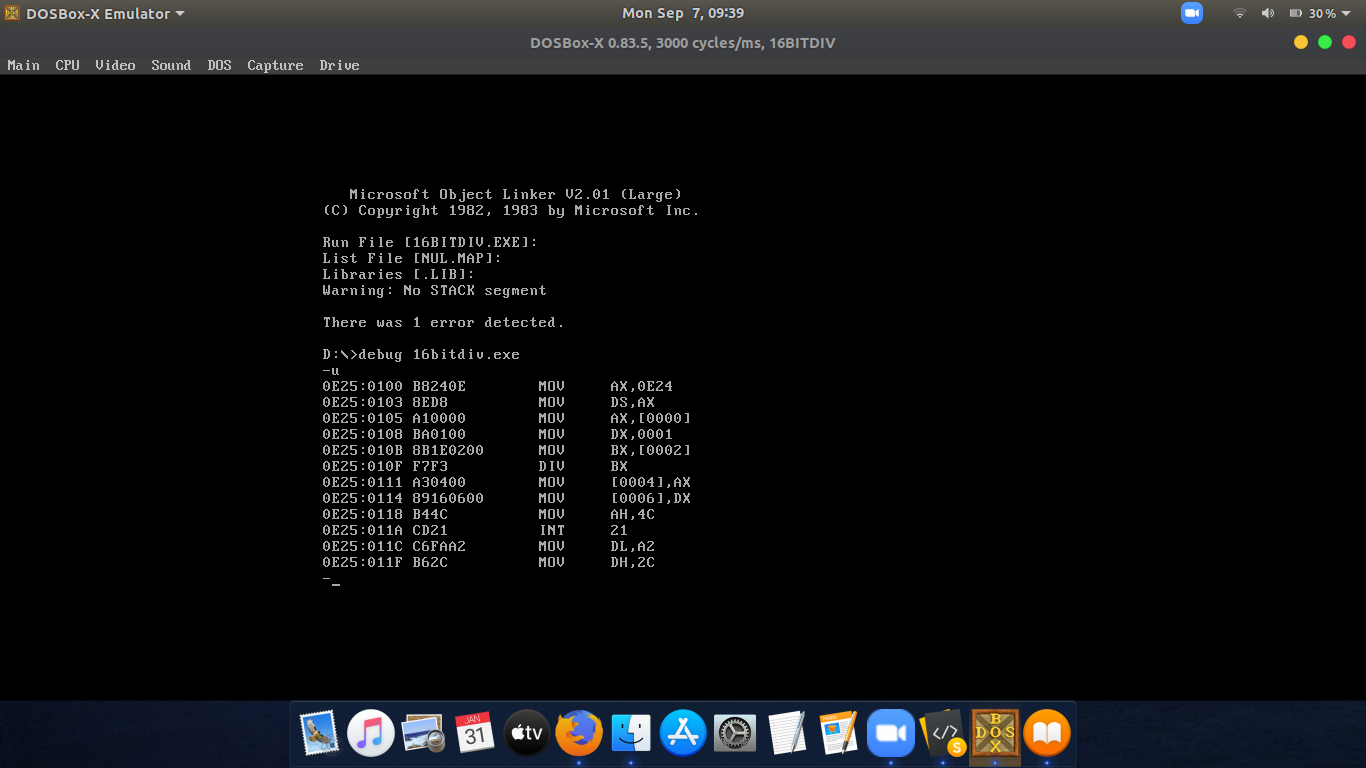
\includegraphics[trim = 100mm 60mm 150mm 127mm, clip, width = \textwidth]{Pics/DivisionUS.png}
\end{figure}
\subsubsection*{\textbf{Input and Output:}}
\begin{figure}[h]
    \centering
    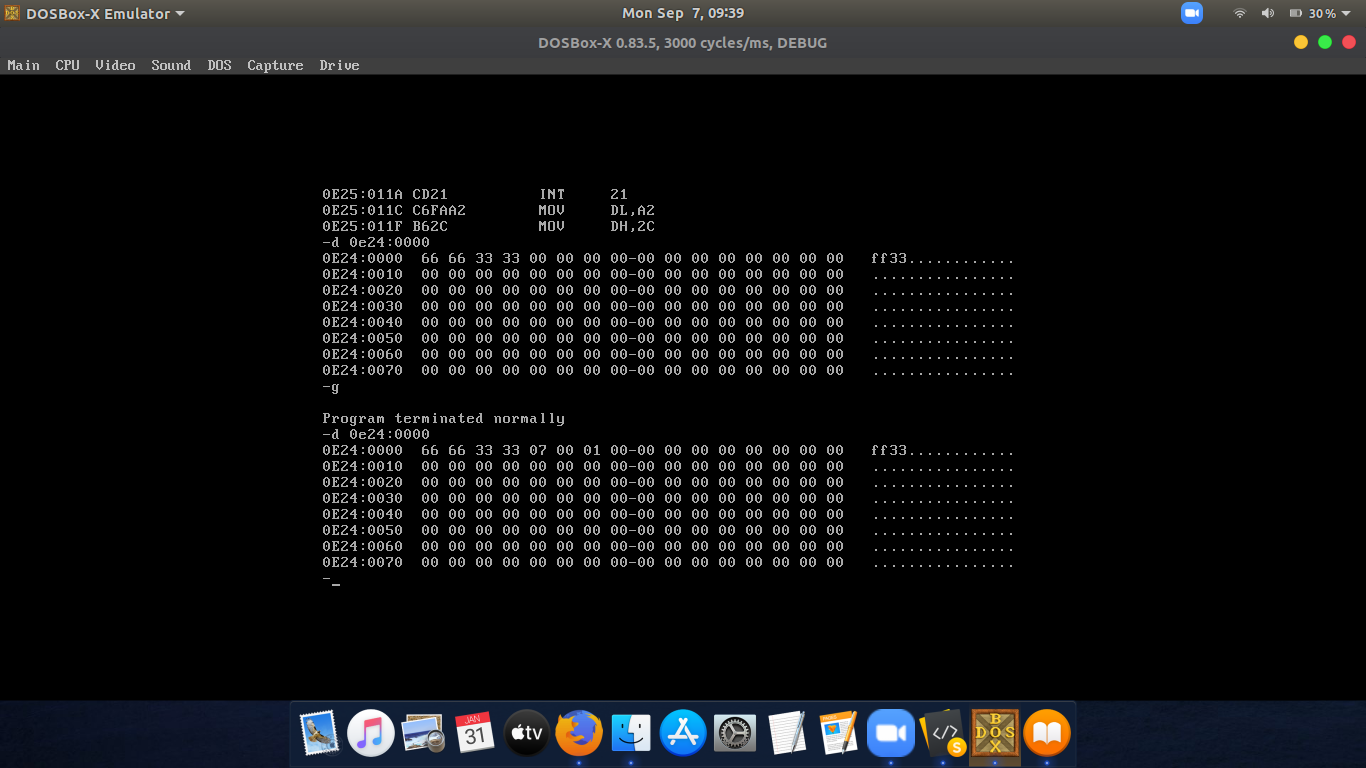
\includegraphics[trim = 100mm 75mm 100mm 70mm, clip, width = \textwidth]{Pics/DivisionIO.png}
    \caption{ \textbf{Input:} \emph{opr1:} 6666h, \emph{opr2:} 3333h; 
              \textbf{Output:} \emph{Quotient:} 0007h, \emph{Remainder:} 0001h}
\end{figure}

\hrule
\subsection*{\textbf{Result:}}
The 8086 programs were written to perform 16-bit arithmetic operations, and the results observed.
\end{flushleft}
\end{document}